\documentclass[a4paper,10pt]{article}
\usepackage[utf8]{inputenc}
\usepackage{dsfont, graphicx}

%opening
\title{Incomplete quantum tomography using neural networks}
\author{Olivia Di Matteo}

\begin{document}

\maketitle

\section{Problem formalism}

The goal of quantum tomography is, given (many identical copies of) some arbitrary quantum state, take a series of measurements in order to determine its density matrix. When the dimension of the system $d$ is prime ($p$), or power of prime ($p^n$), a complete set of $d + 1$ bases that are mutually unbiased comprise an optimal set of measurements. These can be written in vector form, but another common way of expressing them is as $d + 1$ sets of $d - 1$ commuting observables (total of $d^2-1$) which have as mutual eigenvectors bases that are MU.

A density matrix $\rho$ can be expressed in terms of $d^2 - 1$ parameters; while an arbitrary complex $d \times d$ matrix contains $2d^2$ entries, the hermiticity and the condition on the trace of a density matrix, i.e. $\hbox{Tr}(\rho) = 1$ reduce the number of parameters required. A convenient way, for our purposes, is expressing the density matrix in terms of its expansion coefficients in an operator basis:
\begin{equation}
 \rho = \frac{1}{d} \mathds{1} + \frac{1}{d} \sum_{i = 1}^{d^2 - 1} a_i P_i
\end{equation}
\noindent For example, we might choose the Pauli basis, and then this expression is the $d$-dimensional analogue of the 2-dimensional Bloch vector.

The goal of a tomographic process would then be, given some measurement data, to estimate the values of the coefficients $a_i$.

\section{Incomplete tomography using neural networks}

If we consider multi-qubit systems, i.e. $d = 2^n$, the number of measurements required scales poorly with the number of qubits. As larger numbers of qubits become experimentally tractable, we will need effective methods of incomplete tomography to make the reconstruction process feasible. Efforts in this direction have involved compressed sensing, and least-bias maximum-likelihood state estimation (LBMLE). We propose here a method based on neural networks. The idea here is that the networks can be trained to reconstruct states based on simulated incomplete experimental data; this allows the heavy lifting to be done computationally, as one needs only train the network once, and then feed it the ``real'' experimental results. There is also a huge amount of versatility as one can very simply adapt the process to train using whatever measurements are taken in a particular experimental setup.

We propose a very simple feed-forward neural network for this task. 
The network in question is shown in figure \ref{fig:nn}. The input layer consists of the measurement frequencies. These are generated `experimentally' by computing the set of projectors for each of the chosen measurement bases, and the probability of that outcome via the Born rule. Then we use MC simulation to generate frequencies of each outcome. The output layer consists of the basis coefficients above, the $a_i$.

\begin{figure}
 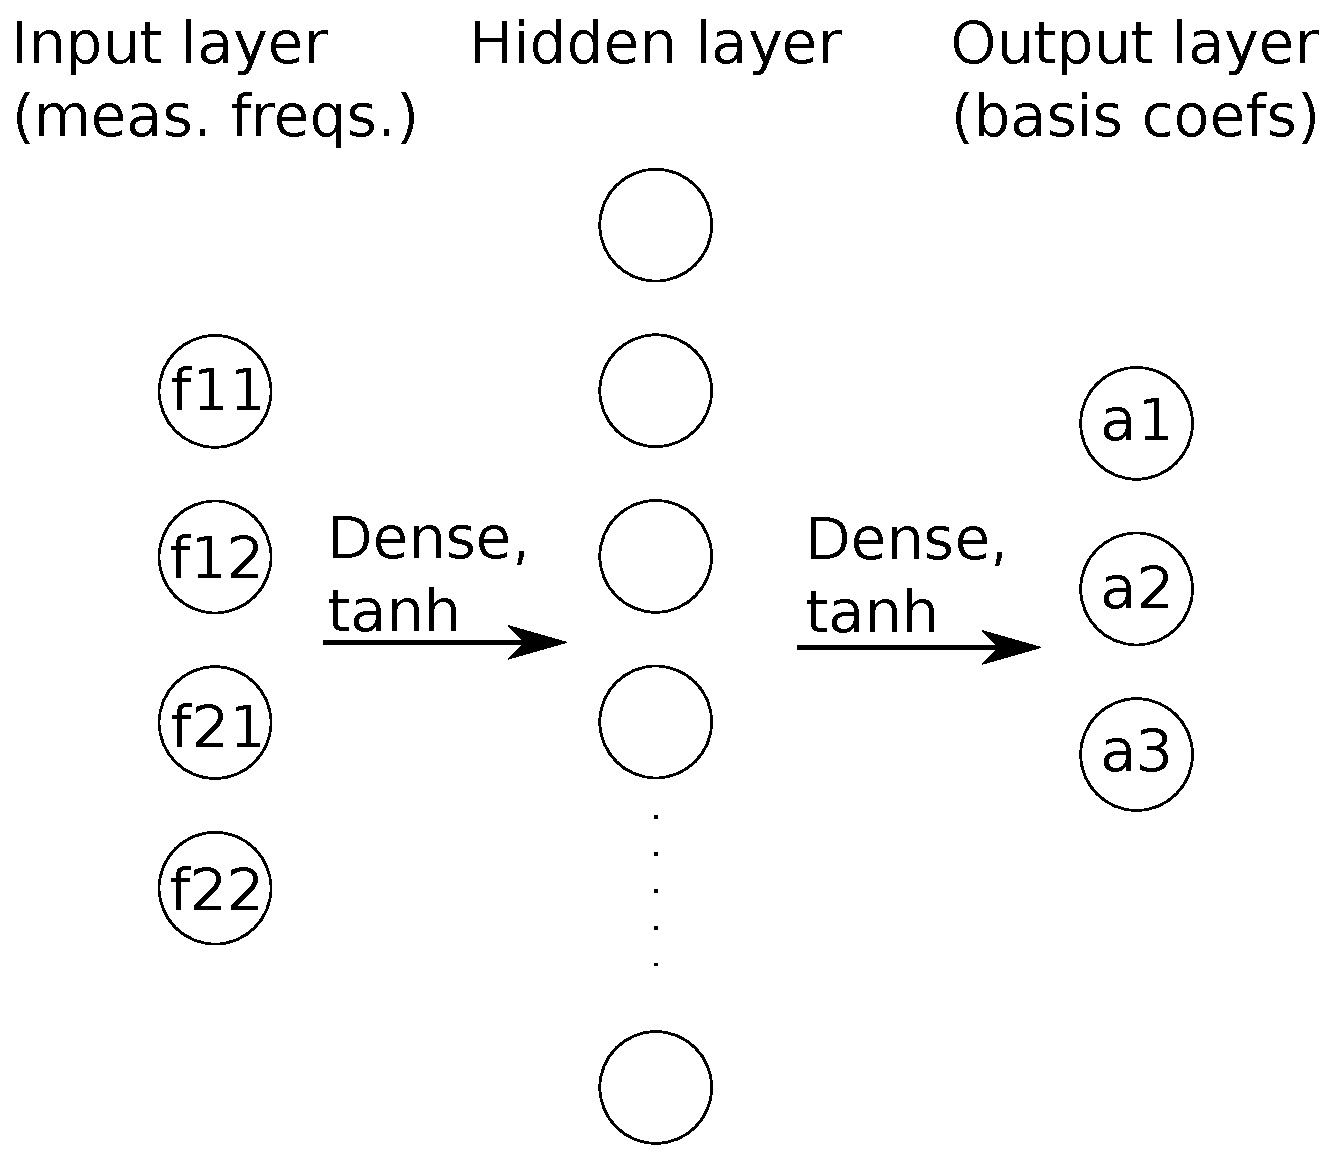
\includegraphics[scale=0.5]{nn_schematic}
 \caption{Simple diagram of neural network. The measurement frequencies from each measured basis are passed in as input nodes. The hidden layer seems to work well with a quadratic number of nodes, after which there are diminishing returns. The output layer should have $d^2 - 1$ nodes.}
 \label{fig:nn}
\end{figure}


In theory this should work great; in practice we need to determine the properties of the hidden layer that are the most effective for this purpose. First, the activation functions. The output vector of coefficients must be normalized, and can contain both positive and negative quantities. We therefore choose tanh as the activation function, as it takes a range (-1, 1). We then manually normalize the output vector so that it is a pure quantum state. For a loss function, we choose the cosine proximity. In essence, this serves to measure the angle between the true and predicted (normalized) vectors; physically, for a single qubit, this would correspond to the angle between vectors on the Bloch sphere, which seems like a sensible thing to try and minimize.


As proof of concept, we have trained the network to reconstruct a single qubit pure state. We trained our network with 9000 Haar-random pure states, and tested on 1000 additional ones. As a metric of success, we choose the fidelity. 

Training the network with all 3 MUBs yields an average fidelity of 0.9999, which is a solid sanity check. We then attempt to train it using simulated measurement data from only 2 of the 3 MUBs.  Our network reconstructs states with a fidelity of 0.944 on average; this can be compared, using the same test data, with the LBMLE algorithm, which reconstructs the states with an average of 0.91.

The distribution of the output fidelities is shown in figure \ref{fig:fids_dim2}. We see that the output of the neural network is more peaked at higher fidelities, whereas that of the LBMLE is more broad.
\begin{figure}
 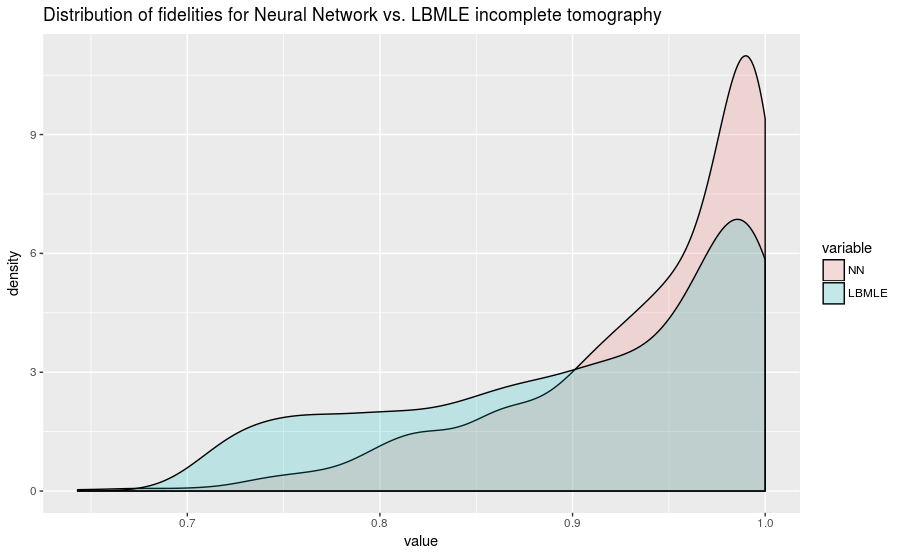
\includegraphics[scale=0.5]{fids_dim2}
 \caption{Density of the output fidelities for reconstruction using neural network vs. LBMLE algorithm. The bases used were the eigenvectors of Pauli $X$ and $Z$.}
 \label{fig:fids_dim2}
\end{figure}


\end{document}
